\begin{frame}
\frametitle{The math}
\begin{itemize}
\item Shannon's entropy: $H(S)= - \sum_{i}{} (p_i*log_2(p_i)$
\vfill
\begin{itemize}
\vfill
\item Higher entropy more information gathered
\end{itemize}
\vfill
\item Example coin toss:
\begin{itemize}
\vfill
\item Entropy = $- P(heads)log_2P(heads)-P(tails)log_2P(tails)$
\vfill
\end{itemize}
\item Information Gain: $IG(A)=H(S)- \sum_{t}{}p(t)H(t)$
\begin{itemize}
\item H(S) = entropy of set S
\item \textit{t} Subset of S obtained by splitting S with A (T)
\item $p(t)$ proportion of elements in t to the no elements in S
\item $H(t)$ entropy of subset t
\end{itemize}
\end{itemize}
\end{frame}

\begin{frame}
\frametitle{Getting to know the data}
Attributes, Classifier, Class features
\begin{center}
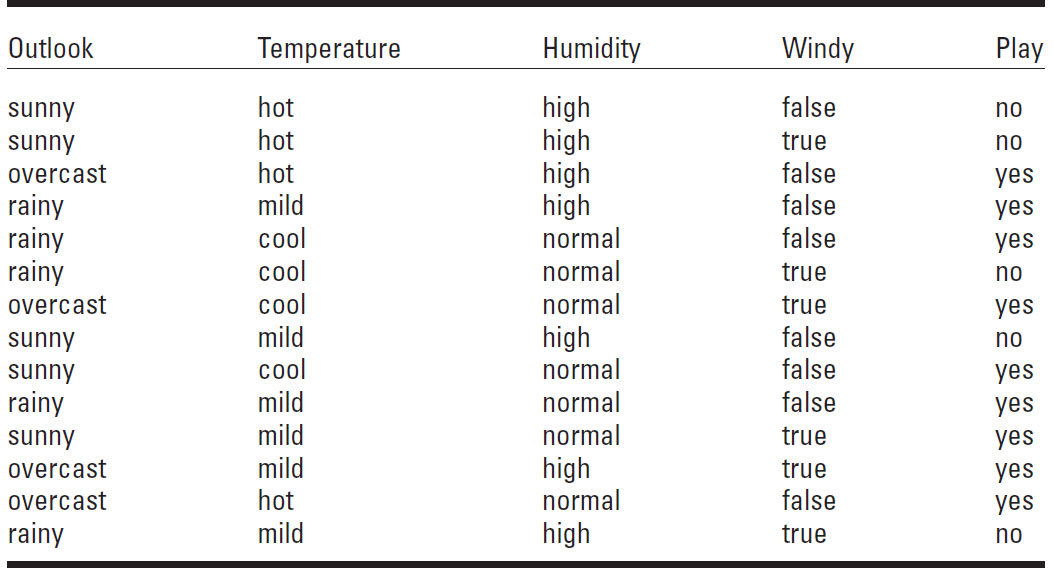
\includegraphics[scale=.3]{Images/tennis.jpg}
\end{center}
\end{frame}

\begin{frame}
\frametitle{Applied math}
\begin{itemize}
\item $Entropy(S)= -\frac{9}{14}log_2(\frac{9}{14})- \frac{5}{14}log_2(\frac{5}{14}) $
\item $Gain(S,Windy) =Entropy(S)-\frac{8}{14}Entropy(S_{false})-\frac{6}{14}Entropy(S_{true})$
\item Windy: 
\begin{itemize}
\item False $8\rightarrow(6_+,2_-)$
\item True $6\rightarrow (3_+,3_-)$
\end{itemize}
\item $Entropy(S_{false})=-\frac{6}{8}log_2(\frac{6}{8})-\frac{2}{8}log_2(\frac{2}{8})$=0.811
\item $Entropy(S_{true})=-\frac{3}{6}log_2(\frac{3}{6})-\frac{3}{6}log_2(\frac{3}{6})$=1
\item $\rightarrow Gain(S,Windy)=0.940-\frac{8}{14}*0.811-\frac{6}{14}*1=0.048$
\item $Gain(S,Humidity)=0.151$ 
\item $Gain(S,Temperature)=0.029$ 
\item $Gain(S,Outlook)=0.246   \leftarrow$ 
\end{itemize}
\end{frame}


\begin{frame}
\frametitle{Stopping}
\begin{itemize}
\item Split the set according to the maximum gain
\item Repeat until homogeneous or pure nodes (ie only leaves or entropy =0)
\end{itemize}
\end{frame}

\begin{frame}
\frametitle{Pseudo-code shamelesly stolen from wikipedia}
\begin{itemize}
	\item If there is a mix of positive and negative examples ID3 works as:
	\item ID3 (Examples, Target Attribute, Attributes)
	\begin{itemize}
	

     \item   A  The Attribute that best classifies examples.
      \item  Decision Tree attribute for Root = A.
      \item  For each possible value, vi, of A,
      \item   Add a new tree branch below Root, corresponding to the test A = vi.
       \item Let Examples(vi) be the subset of examples that have the value vi for A
      \item If Examples(vi) is empty
     \item   New branch and add a leaf node with label = most common target value in the examples
   \item  Else branch and add the subtree ID3 (Examples(vi), Target Attribute, Attributes – {A})
   \item  End
   \item  Return Root

	\end{itemize}
		\end{itemize}


\end{frame}